\chapter{All'opera}
\epigraph{Tutto ciò che è bello e nobile è il risultato della ragione e di calcoli.}{Baudelaire}

In questo capitolo verranno affrontati i principali passaggi per arrivare a dati utilizzabili per calcolare le probabilità, come richiesto dall'equazione \eqref{prob_finale}.

\section{Download del dataset di Wikipedia}
\label{dump}
Wikipedia è una sorgente di dati ben nota nell'ambito della ricerca sull'NLP. All'indirizzo \url{http://dumps.wikimedia.org/} la Wikimedia Foundation ospita una serie di file pronti al download, generati periodicamente da bot, che consentono di reperire con più facilità i dati quando si tratta di una grande mole. In questo particolare scenario l'utilizzo delle API (si veda il paragrafo \ref{wikiapi}) è fortemente sconsigliato in quanto genera un inutile overload sui server e risulta comunque più lento rispetto al primo metodo.

All'indirizzo \url{http://dumps.wikimedia.org/itwiki/} sono ospitati i dump relativi alla versione italiana di Wikipedia. La base da cui si è partiti è la versione \texttt{20150316} nella variante che comprende tutte le pagine correnti, senza cronologia e senza file multimediali associati. La scelta è stata fatta sia per avere una dimensione dei dati gestibile (al momento della stesura il dump indicato ha una dimensione di circa $\SI{2}{\giga\byte}$) sia per avere dati sempre ``freschi'': non avrebbe senso fare statistica su un testo che gli utenti hanno già corretto, migliorato o comunque rivisto.

\section{Dal dataset al plaintext}

Il dataset è compresso in formato \texttt{bzip2}. Per decomprimerlo è sufficiente eseguire da riga di comando:
\indent{\shellcmd{tar xjf itwiki-20150316-pages-articles.xml.bz2}}
Verrà creato un file XML che contiene il testo di tutte le pagine insieme ad alcune informazioni aggiuntive (i cosiddetti \emph{metadati}, per esempio l'autore originale, la data di creazione e quella di ultima modifica, la categoria, \dots).
Nel tag \texttt{<text>} è contenuto il testo sorgente della pagina codificato in un miscuglio di HTML e XML (``MediaWiki Markup Language'') che rende difficile il parsing. Poiché a noi interessa solo testo in chiaro senza informazioni ulteriori, tra i vari progetti disponibili possiamo sfruttare \emph{Wikipedia Extractor} \cite{WikiExtractorUniPi}, un lavoro di alcuni ricercatori dell'Università di Pisa che ``ripulisce'' il contenuto della pagina.

Wikipedia in lingua italiana è una grossa enciclopedia con oltre un milione di voci: è quindi fondamentale che l'elaborazione dei dati avvenga in tempi accettabili. Il lodevole progetto dell'Università di Pisa è stato quindi migliorato da un altro studente che ne ha realizzato una versione multithread \cite{WikiExtractorMTUniPi}, sfruttando a pieno la grande potenza computazionale delle CPU odierne. Sulla postazione utilizzata per lo sviluppo di questo progetto, equipaggiata con un processore ad 8 core, si è osservato un incremento prestazionale circa del 600\%.

Nel corso del progetto lo script è stato migliorato nei seguenti aspetti:
\begin{itemize}
	\item Aggiunta la modalità di output in plaintext.
	\item Aggiunta la possibilità di specificare il numero di thread da utilizzare.
	\item Aggiunta la possibilità di specificare il nome dell'unico file di output (in origine era prevista una cartella con file divisi e rinominati casualmente).
	\item Lievi miglioramenti al supporto UTF-8.
	\item Revisione completa dello script per la piena compatibilità con lo standard di scrittura codice Python PEP8.
\end{itemize}

Quest'ultima versione è disponibile nel repository pubblico del progetto (cfr. \ref{pubb}).
\section{Dal plaintext agli N-grammi}
Come si è visto nel capitolo \ref{cap_teoria}, per raccogliere statistiche usabili nel determinare il ``language model'' abbiamo bisogno delle frequenze con cui unigrammi e bigrammi appaiono nel testo appena estratto. Questo compito soffre naturalmente degli stessi problemi di quello precedente: abbiamo bisogno di uno script che faccia il proprio lavoro in tempi ragionevoli e con un consumo di memoria accettabile.

La prima versione del programma realizzato svolgeva egregiamente il suo compito limitatamente a input di modeste dimensioni; si scontrava invece con il limite della memoria RAM disponibile sulla macchina di sviluppo ($\SI{8}{\gibi\byte}$) quando eseguito con input più consistenti.
Al fine di migliorare l'efficienza della soluzione si è intervenuti su alcuni fronti:
\begin{itemize}
\item L'esecuzione del codice è stata resa parallela. Ciò comporta non pochi problemi in Python, in quanto la maggior parte delle implementazioni degli interpreti usano GIL\footnote{Global Interpreter Lock. È un meccanismo di sincronizzazione usato nei linguaggi interpretati che regola l'esecuzione di thread multipli affinché ne venga eseguito solo uno alla volta.} rendendo inutile l'uso dei thread. Si è quindi fatto ricorso alla creazione di processi figli (analogamente a quanto avviene in C con l'istruzione \texttt{fork()}) a cui si demanda il calcolo delle frequenze delle parole. L'architettura complessiva prevede quindi un processo che legge il file in ingresso una riga alla volta. Ciascuna riga diventa un ``compito'' da svolgere e viene messa in una coda che viene via via svuotata dai vari processi (worker). Quando la coda 1 è vuota, i worker terminano il loro lavoro e salvano i risultati nella coda 2, che verrà elaborata da un altro processo. Quest'ultimo unisce i risultati parziali calcolando le frequenze totali che vengono scritte in un file di output.
\begin{figure}[h]
\centering
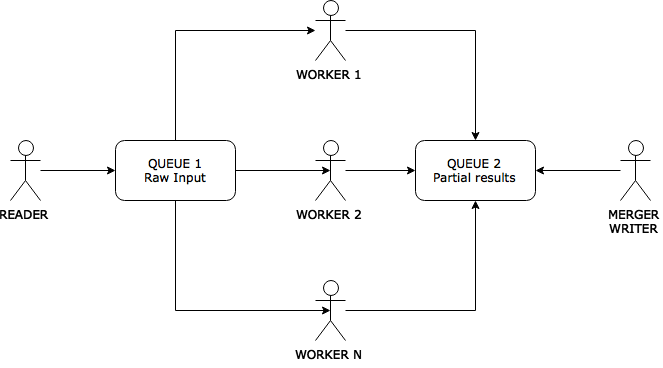
\includegraphics[width=\textwidth]{Figures/computeFrequencies.png}
\caption{Schema logico di computeFrequencies.py}
\end{figure}
\item Il codice del progetto è stato migrato alla versione 3.4 di Python che include un'interessante funzionalità: i dizionari a chiave condivisa\footnote{\url{https://www.python.org/dev/peps/pep-0412/}}. Questa caratteristica consente all'interprete Python di allocare memoria una sola volta per memorizzare le chiavi dei dizionari tra più istanze della stessa classe. Poiché lo script prevede una classe per rappresentare un processo e \texttt{Counter}, la classe utilizzata per contare le frequenze, è derivata dalla classe dizionario, questa modifica porta un significativo miglioramento del consumo di RAM dello script. Da alcuni test di verifica, il risparmio di memoria si è mostrato superiore al 50\%.
\item Nonostante la miglioria precedente, per il calcolo di tutte le frequenze dei bigrammi lo script richiede un quantitativo di RAM superiore a quello disponibile nella macchina di sviluppo. Si è quindi scelto di eseguirlo su una macchina virtuale Amazon EC2 di tipo \texttt{c3.2xlarge} con 8 CPU virtuali e $\SI{15}{\gibi\byte}$ di RAM. Il programma ha quindi svolto il suo compito in 1018 secondi (circa 17 minuti), con un picco di occupazione RAM intorno ai $\SI{13}{\gibi\byte}$.
\end{itemize}

\section{Scelta del DBMS}
\label{dbms}
Le occorrenze calcolate sono memorizzate in file con la seguente sintassi:

\indent{\texttt{Ngramma Frequenza}}

Le frequenze sono quindi da memorizzare in una base di dati che conservi queste coppie (chiave, valore) e ne consenta l'interrogazione in modo estremamente efficiente. Per stabilire infatti la migliore correzione possibile per una parola, come abbiamo visto nel capitolo \ref{cap_teoria}, è necessario calcolare un grande numero di probabilità. Per questo il DBMS Redis\footnote{\url{http://redis.io/}} fa al caso nostro \cite{nltkredis}. Redis è un database NoSQL ultra efficiente per memorizzare nella RAM coppie chiave-valore, che possono facoltativamente essere salvate su disco per garantire la persistenza. 

Le prestazioni di Redis variano, come è ovvio, dalla potenza dell'host su cui il server è installato ma anche dalla tipologia di connessione tra client e server (via TCP oppure UNIX socket). In linea di massima è comunque possibile affermare che Redis è in grado di servire oltre 100\,000 query/s.

Poiché per sua natura Redis mantiene tutte le informazioni direttamente in memoria è imporante che il server sia dimensionato correttamente in termini di RAM. In particolare, per questa installazione che contiene tutti gli unigrammi e i bigrammi il processo \texttt{redis-server} occupa (a caricamento completato) circa $\SI{1,7}{\gibi\byte}$.
La soluzione scelta per la produzione è su una VPS dedicata allo scopo con $\SI{2}{\gibi\byte}$ di RAM, disco SSD e connettività a $\SI{1}{GBps}$.

	\begin{mdframed}[style=indepth]
		\begingroup
		\setlength{\fboxsep}{0pt}%  
		\colorbox{black!50!white}{\makebox[\linewidth]{\textcolor{white}{\parbox[c][.8cm][c]{\linewidth}{\centering\textsc{A look into the world of NoSQL databases}}}}}
		\endgroup
		\hrule\vspace*{2mm}
		\hspace{.03\linewidth}\begin{minipage}{.94\linewidth}
NoSQL databases provide a mechanism for storing and retrieving data that is memorized in a different way than the tabular relations used in relational DBs. 

NoSQL databases are designed in contrast to relational databases, which were first introduced by Codd, an English computer scientist. He used the definition of a mathematical relation to organize data into one or more tables of rows and columns.

NoSQL databases feature highly optimized key-value operations (i.e., storing and reading a value given a key). Datastore of this kind may not require fixed table schemas and usually avoid join operations.

The term gained popularity in early 2009 with the advent of big data. In fact NoSQL DBs are often employed in real-time web applications and those requiring fast computation of a huge amount of data.
The benefits include:
\begin{itemize}
\item Scalability and superior performances;
\item Capability to memorize large volumes of structured and unstructured data;
\item An efficient architecture that can easily scale out;
\item Most implementations are open source.
\end{itemize}
Instead, the downsides are:
\begin{itemize}
\item Immaturity;
\item No support for a well-known and standardized language, as SQL;
\item No ACID transactions;
\item Many data structures (objects) cannot be easily represented as key-value pairs without a complex serialization.
\end{itemize}
		\end{minipage}
	\end{mdframed}


\section{Aggiornamenti in tempo reale}
Per fare in modo che il sistema proposto migliori con il tempo proponiamo una soluzione che migliori costantemente la base di dati su cui lavora l'algoritmo. Come già spiegato, tutto il lavoro di correzione si basa sulle probabilità ottenute dall'elaborazione di Wikipeida. La sorgente di dati non è stata scelta a caso: Wikipedia è continuamente aggiornata dagli utenti che correggono (inevitabili) errori e aggiungono contenuti.
Aggiornando quindi il nostro database i dati in esso contenuti vengono continuamente raffinati e, speranzosamente, offriranno una qualità della correzione sempre migliore.

\subsection{MediaWiki API}
\label{wikiapi}
Wikipedia, oltre al servizio di dump descritto nel paragrafo \ref{dump}, offre anche un insieme di API che consente a bot e terze parti di recuperare ed eventualmente modificare i dati. Il servizio di API, per la versione italiana, è disponibile presso \url{http://it.wikipedia.org/w/api.php}. Esistono diversi wrapper per l'API, ma spesso sono incompleti e poco aggiornati rispetto alle ultime versioni dell'interfaccia. Pertanto è stata creata una nuova classe Python che astrae l'interfaccia offrendo due metodi:
\begin{itemize}
\item \texttt{getRecentChanges}: restituisce una lista di (al più 500) oggetti JSON dove ciascuno rappresenta una modifica a una pagina di Wikipedia. È possibile specificare anche la data e l'ora da cui partire a recuperare le modifiche.
\item \texttt{getPageReviews}: a partire da una lista di identificativi di revisione, recupera il testo di ciascuna delle pagine a cui le revisioni fanno riferimento prima e dopo di esse.
\end{itemize}
La classe è disponibile nel repository del progetto.
